\documentclass{article}
\usepackage[utf8]{inputenc}
\usepackage{geometry}
\usepackage{pdfpages}
\usepackage{graphicx}
\usepackage{filecontents}

\graphicspath{{images/}}
\geometry{
	a4paper,
	total={170mm,257mm},
	left=20mm,
	top=20mm,
}
\usepackage{graphicx}
\usepackage{titling}
\usepackage[american,RPvoltages]{circuiTikz}
\usepackage{tikz, tikz-cd}
\usepackage{pgfplots}
\usepackage{siunitx}
\usepackage{float}
\usepackage{enumitem}
\usepackage{amsmath,amsfonts,stmaryrd,amssymb} % Math packages
\usepackage{schemabloc}
\usepackage{tcolorbox}
\usetikzlibrary{circuits}
\usetikzlibrary{positioning}
\title{Filtro Capacitivo}
\author{Rodrigo Castillejos}
\date{Agosto 2024}

\usepackage{fancyhdr}
\fancypagestyle{plain}{%  the preset of fancyhdr 
	\fancyhf{} % clear all header and footer fields
	\fancyfoot[L]{\thedate}
	\fancyhead[L]{Filtro Capacitivo}
	\fancyhead[R]{\theauthor}
}
\makeatletter
\def\@maketitle{%
	\newpage
	\null
	\vskip 1em%
	\begin{center}%
		\let \footnote \thanks
		{\LARGE \@title \par}%
		\vskip 1em%
		%{\large \@date}%
	\end{center}%
	\par
	\vskip 1em}
\makeatother

\usepackage{lipsum}  
\usepackage{cmbright}

\begin{document}
	
	\maketitle
	
	\noindent\begin{tabular}{@{}ll}
		Autor & \theauthor\\
		Tema &  Circuitos Eléctricos\\
	\end{tabular}
	
	\section*{Filtro capacitivo}
	Un capacitor es un elemento de almacenamiento de energía, éste intenta mantener un voltaje constante, previniendo por lo tanto cualquier cambio de voltaje a través de la carga. Un capacitor $C$ puede conectarse en paralelo con la carga para mantener un voltaje continuo de salida constante $v_o$ como se muestra en la figura 1. Bajo condiciones de estado estable, el capacitor tendrá un voltaje finito inicial. Cuando el voltaje instantáneo de la magnitud de la fuente de alimentación $v_S$ sea mayor que el voltaje instantáneo del capacitor $v_C$, los diodos ($D_1$ y $D_2$ o $D_3$ y $D_4$) conducirán y el capacitor se cargará a través de la fuente de entrada. 
	
	\begin{figure}[H]
	\centering	
	\begin{tikzpicture}[scale=0.8, voltage shift=1]
		\draw (0,0) ++(2.5,0) coordinate(n0) to[D*, l=$D_4$] ++(0,4) coordinate(n1)
		to[sV, l=$V_s$, f<^=$i_S$] ++(4,0) coordinate(n2)
		to[D*, invert, l=$D_2$, -*] ++(0,-4) coordinate(n4)
		to[short] ++(-4,0);
		\draw (n1)  to[D*,l=$D_1$, *-] ++(0,4)
		to[short] ++(4,0) coordinate(n3)
		to[D*, invert, l=$D_3$, -*] (n2);
		\draw (n3)  to[short, *-] ++(4,0) coordinate(n5) 
		to[C, v=$v_c$, l=$C$, -*] (n5 |- n4) coordinate(n7) -- (n4);
		\draw (n5)  to[short, f=$i_O$, *-] ++(4,0) coordinate(n6)
		to[R, l_=$R_L$, v^={$v_O = v_C$}] (n6 |- n7) coordinate(n11) -- (n7);
		\coordinate (M) at ($(n0)!0.5!(n11)$);
		\draw (M) node[below=0.2cm]{$(a) \, circuito$};
		\draw (0,0) ++(0,-6) coordinate(p1) to[sV, l=$V_s$] ++(0,4)
		to[D*, l=$D_1$] ++(3,0)
		to[D*, l=$D_2$] ++(3,0) coordinate(n8)
		to[C, -*, v=$v_C$, l=$C$] ++(0,-4) coordinate(n9)
		to[short] ++(-6,0);
		\draw (n8)  to[short, *-, f=$i_O$] ++(4,0) coordinate(n10)
		to[R, l=$R_L$] (n10 |- n9) coordinate(p2) -- (n9);
		\coordinate (M1) at ($(p1)!0.5!(p2)$);
		\draw (M1) node[below=0.2cm]{$(b) \, carga$};
		\draw (n10) ++(3,0) to[short, f=$i_O$] ++(4,0)
		to[R, l=$R_L$] ++(0,-4) coordinate(p3)
		to[short] ++(-4,0) coordinate(p4)
		to[C, l=$C$, v>=$v_m$] ++(0,4);
		\coordinate (M2) at ($(p3)!0.5!(p4)$);
		\draw (M2) node[below=0.2cm]{$(c) \, descarga$};
	\end{tikzpicture}
	\caption{}	
	\label{fig:figura1}
\end{figure}


	\noindent Sin embargo, si la magnitud del voltaje $v_S$ cae por debajo del voltaje instantáneo del capacitor C los diodos ($D_1$ y $D_2$ o $D_3$ y $D_4$) estarán polarizados en inversa y el capacitor C se descargará a través de la resistencia de carga $R_L$. El voltaje del capacitor $v_C$ variará entre un valor mínimo $V_{o(min)}$ y un valor máximo $V_{o(max)}$. Las formas de onda del voltaje de salida $v_O$ y el voltaje de rizado $v_r$ se muestran en la figura 2. Si $f$ es la frecuencia de la fuente de entrada, entonces el periodo del voltaje de entrada es $T=1/f$.
	
	\begin{figure}[H]
	\centering
	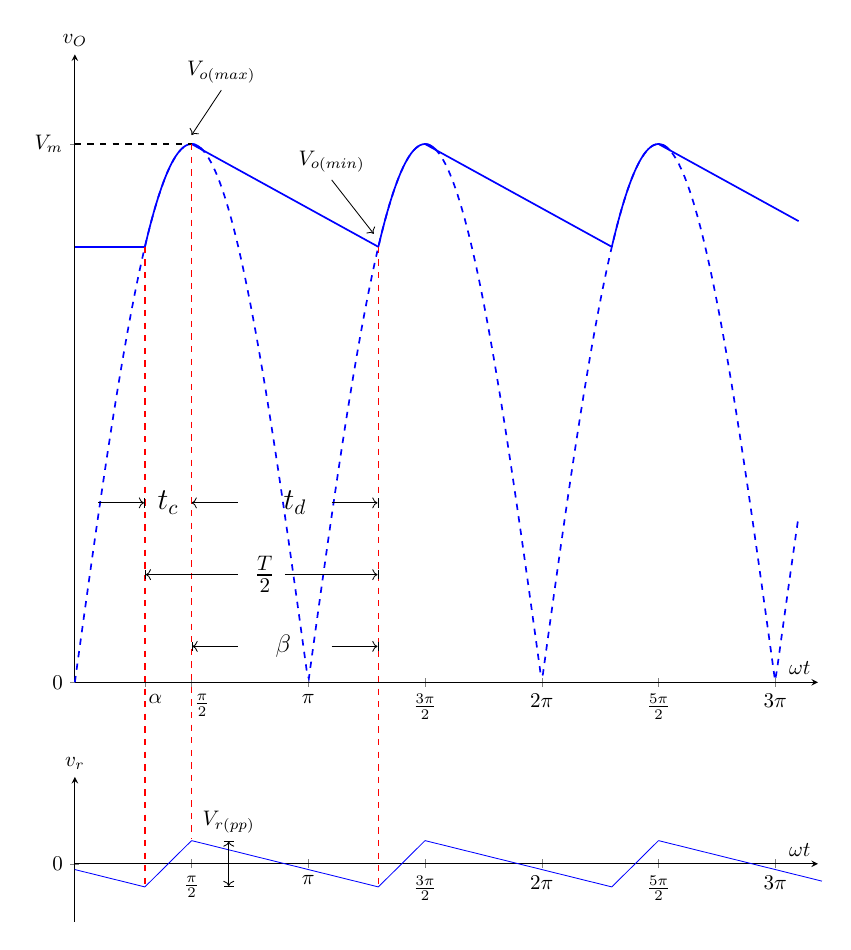
\begin{tikzpicture}[scale=0.76, remember picture]
		\pgfplotsset{width=14cm,compat=1.18}
		\begin{axis}[
			name=plot1,
			clip=false,
			axis y line=left,
			axis x line=middle,
			xlabel=$\omega t$,
			ymin=0, ymax=3.5,
			xmin=0, xmax=10,
			domain=0:3.5*pi,
			samples=400,
			xtick={0, 0.3*pi, 1.5708, 3.14159, 4.7123889,6.28318, 7.85398, 9.42477},
			xticklabels={$0$,$\,\,\,\,\,\, \alpha$,$\,\,\,\,\,\, \frac{\pi}{2}$, $\pi$, $\frac{3\pi}{2}$, $2\pi$, $\frac{5\pi}{2}$, $3\pi$},
			ytick={0, 3},
			yticklabels={$0$,$V_m$}]
			\addplot[mark=none, blue, domain=0:3.1*pi, thick=0.6, dashed] {3*abs(sin(deg(x)))};
			\addplot[mark=none, blue, domain=0.3*pi:0.55*pi, thick=0.6] {3*abs(sin(deg(x)))};
			\addplot[mark=none, blue, domain=0:0.3*pi, thick=0.6] {2.427};
			\addplot[mark=none, blue, domain=0.5*pi:1.3*pi, thick=0.6] {-0.22799*(x-pi/2) + 3};
			\addplot[mark=none, blue, domain=1.3*pi:1.55*pi, thick=0.6] {3*abs(sin(deg(x)))};
			\addplot[mark=none, blue, domain=1.5*pi:2.3*pi, thick=0.6] {-0.22799*(x-1.5*pi) + 3};
			\addplot[mark=none, blue, domain=2.3*pi:2.55*pi, thick=0.6] {3*abs(sin(deg(x)))};
			\addplot[mark=none, blue, domain=2.5*pi:3.1*pi, thick=0.6] {-0.22799*(x-2.5*pi) + 3};
			\draw (0,3.5) node[above]{$v_O$}; 
			\addplot[color = black, thick, dashed] coordinates {(0,3) (pi/2,3)}; %horizontal1
			\addplot[color = red, dashed, thick] coordinates {(0.3*pi,2.427) (0.3*pi,-1.15)}; %vertical1
			\addplot[color = red, dashed, thick] coordinates {(pi/2,3) (pi/2,-0.87)}; %vertical2
			\addplot[color = red, dashed, thick] coordinates {(1.3*pi,2.427) (1.3*pi,-1.15)}; %vertical3
			\draw[<-](pi/2, 3.05)--(pi/2 + 0.4, 3.3); %vo_max
			\node[above] at (axis cs:1.970796,3.3){$V_{o(max)}$};
			\draw[<-](1.28*pi, 2.5)--(1.1*pi, 2.8); %vo_min
			\node[above] at (axis cs:1.1*pi, 2.8){$V_{o(min)}$};
			\draw[->|] (0.1*pi,1) -- (0.3*pi,1) node[right=0.9mm]{{\Large $t_c$}};
			\draw[<-] (0.5*pi,1) -- (0.7*pi,1);
			\draw[->|] (1.1*pi,1) node[left=3mm]{{\Large $t_d$}} -- (1.3*pi,1);
			\draw[|<-] (0.3*pi,0.6) -- (0.7*pi,0.6) node[right=1.5mm]{{\Large $\frac{T}{2}$}};
			\draw[->|] (0.9*pi,0.6) -- (1.3*pi,0.6);
			\draw[|<-] (0.5*pi,0.2) -- (0.7*pi,0.2) node[right=5mm]{{\large $\beta$}};
			\draw[->|] (1.1*pi,0.2) -- (1.3*pi,0.2);
		\end{axis}
		
	    \pgfplotsset{width=14cm,compat=1.18}
		\begin{axis}[
			yshift=-4cm,
			clip=false,
			name=plot2,
			height=4cm,
			%at=(plot1.below south west), anchor=above north west,
			axis y line=left,
			axis x line=middle,
			ymin=-1, ymax=1.5,
			xmin=0, xmax=10,
			domain=0:3.5*pi,
			samples=200,
			xlabel=$\omega t$,
			xtick={0, 1.5708, 3.14159, 4.7123889,6.28318, 7.85398, 9.42477},
			xticklabels={$0$,$\frac{\pi}{2}$, $\pi$, $\frac{3\pi}{2}$, $2\pi$, $\frac{5\pi}{2}$, $3\pi$},
			ytick={0},
			%yticklabels={$0$,$V_m$}]
			]
			\addplot[mark=none, blue, domain=0:0.3*pi] {((-0.4-0.4)/(0.3*pi +0.5*pi))*(x + 0.5*pi) + 0.4};
			\addplot[mark=none, blue, domain=0.3*pi:0.5*pi] {((0.4+0.4)/(0.5*pi - 0.3*pi))*(x - 0.3*pi) - 0.4};
			\addplot[mark=none, blue, domain=0.5*pi:1.3*pi] {((-0.4-0.4)/(1.3*pi - 0.5*pi))*(x - 0.5*pi) + 0.4};
			\addplot[mark=none, blue, domain=1.3*pi:1.5*pi] {((0.4+0.4)/(1.5*pi - 1.3*pi))*(x - 1.3*pi) - 0.4};
			\addplot[mark=none, blue, domain=1.5*pi:2.3*pi] {((-0.4-0.4)/(2.3*pi - 1.5*pi))*(x - 1.5*pi) + 0.4};
			\addplot[mark=none, blue, domain=2.3*pi:2.5*pi] {((0.4+0.4)/(2.5*pi - 2.3*pi))*(x - 2.3*pi) - 0.4};
			\addplot[mark=none, blue, domain=2.5*pi:3.2*pi] {((-0.4-0.4)/(3.3*pi - 2.5*pi))*(x - 2.5*pi) + 0.4};
			\node[above] at (axis cs:0,1.5){$v_r$};
			\draw[|<->|] (0.5*pi + 0.5,0.4) node[above]{$V_{r(pp)}$} -- (0.5*pi + 0.5,-0.4) ;
		\end{axis}
	\end{tikzpicture}
	\caption{}	
	\label{fig:figura2}
\end{figure}

	\begin{figure}[H]
	\centering
	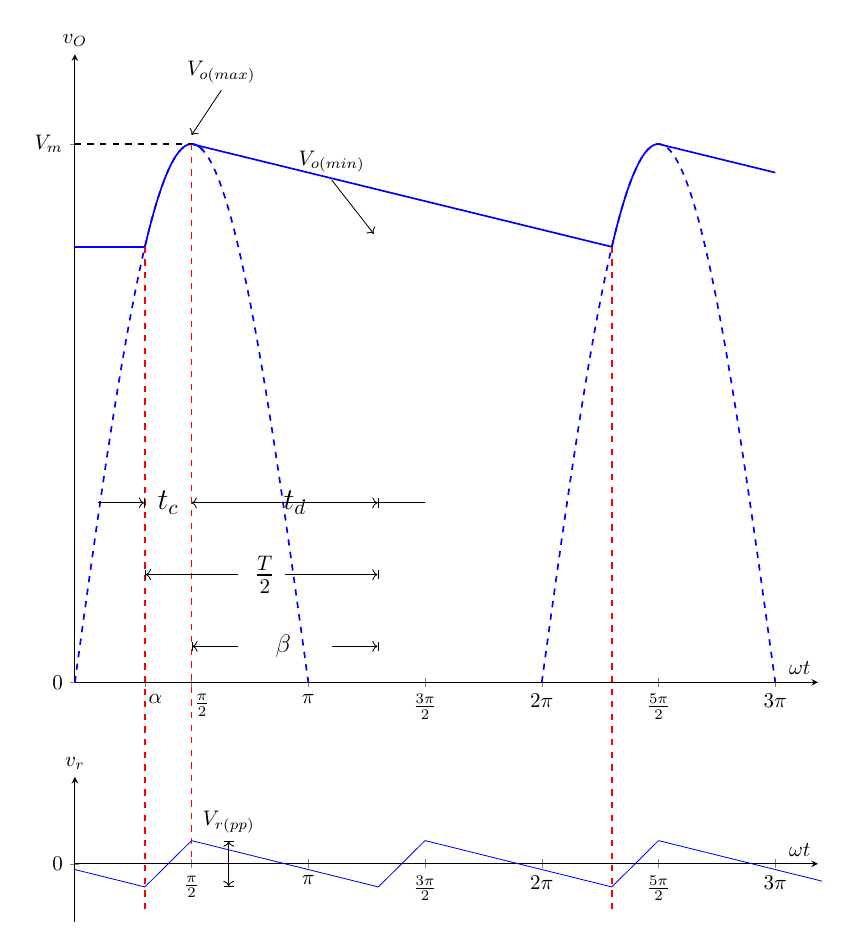
\begin{tikzpicture}[scale=0.76, remember picture]
		\pgfplotsset{width=14cm,compat=1.18}
		\begin{axis}[
			name=plot1,
			clip=false,
			axis y line=left,
			axis x line=middle,
			xlabel=$\omega t$,
			ymin=0, ymax=3.5,
			xmin=0, xmax=10,
			domain=0:4.5*pi,
			samples=400,
			xtick={0, 0.3*pi, 1.5708, 3.14159, 4.7123889,6.28318, 7.85398, 9.42477, 4*pi},
			xticklabels={$0$,$\,\,\,\,\,\, \alpha$,$\,\,\,\,\,\, \frac{\pi}{2}$, $\pi$, $\frac{3\pi}{2}$, $2\pi$, $\frac{5\pi}{2}$, $3\pi$,$4\pi$},
			ytick={0, 3},
			yticklabels={$0$,$V_m$}]
			\addplot[mark=none, blue, domain=0:pi, thick=0.6, dashed] {3*abs(sin(deg(x)))};
			\addplot[mark=none, blue, domain=2*pi:3*pi, thick=0.6, dashed] {3*abs(sin(deg(x)))};
			\addplot[mark=none, blue, domain=0.3*pi:0.55*pi, thick=0.6] {3*abs(sin(deg(x)))};
			\addplot[mark=none, blue, domain=0:0.3*pi, thick=0.6] {2.427};
			\addplot[mark=none, blue, domain=0.5*pi:2.3*pi, thick=0.6] {-0.101328*(x - 0.5*pi) + 3};
			\addplot[mark=none, blue, domain=2.3*pi:2.5*pi, thick=0.6] {3*sin(deg(x))};
			\addplot[mark=none, blue, domain=2.5*pi:*3*pi, thick=0.6] {-0.101328*(x - 0.5*pi - 2*pi) + 3};
			\draw (0,3.5) node[above]{$v_O$}; 
			\addplot[color = black, thick, dashed] coordinates {(0,3) (pi/2,3)}; %horizontal1
			\addplot[color = red, dashed, thick] coordinates {(0.3*pi,2.427) (0.3*pi,-1.3)}; %vertical1
			\addplot[color = red, dashed, thick] coordinates {(pi/2,3) (pi/2,-1.02)}; %vertical2
			\addplot[color = red, dashed, thick] coordinates {(2.3*pi,2.427) (2.3*pi,-1.3)}; %vertical3

			\draw[<-](pi/2, 3.05)--(pi/2 + 0.4, 3.3); %vo_max
			\node[above] at (axis cs:1.970796,3.3){$V_{o(max)}$};
			\draw[<-](1.28*pi, 2.5)--(1.1*pi, 2.8); %vo_min
			\node[above] at (axis cs:1.1*pi, 2.8){$V_{o(min)}$};
			\draw[->|] (0.1*pi,1) -- (0.3*pi,1) node[right=0.9mm]{{\Large $t_c$}};
			\draw[<-] (0.5*pi,1) -- (1.5*pi,1);
			\draw[->|] (1.1*pi,1) node[left=3mm]{{\Large $t_d$}} -- (1.3*pi,1);
			\draw[|<-] (0.3*pi,0.6) -- (0.7*pi,0.6) node[right=1.5mm]{{\Large $\frac{T}{2}$}};
			\draw[->|] (0.9*pi,0.6) -- (1.3*pi,0.6);
			\draw[|<-] (0.5*pi,0.2) -- (0.7*pi,0.2) node[right=5mm]{{\large $\beta$}};
			\draw[->|] (1.1*pi,0.2) -- (1.3*pi,0.2);
		\end{axis}
		
		\pgfplotsset{width=14cm,compat=1.18}
		\begin{axis}[
			yshift=-4cm,
			clip=false,
			name=plot2,
			height=4cm,
			%at=(plot1.below south west), anchor=above north west,
			axis y line=left,
			axis x line=middle,
			ymin=-1, ymax=1.5,
			xmin=0, xmax=10,
			domain=0:3.5*pi,
			samples=200,
			xlabel=$\omega t$,
			xtick={0, 1.5708, 3.14159, 4.7123889,6.28318, 7.85398, 9.42477},
			xticklabels={$0$,$\frac{\pi}{2}$, $\pi$, $\frac{3\pi}{2}$, $2\pi$, $\frac{5\pi}{2}$, $3\pi$},
			ytick={0},
			%yticklabels={$0$,$V_m$}]
			]
			\addplot[mark=none, blue, domain=0:0.3*pi] {((-0.4-0.4)/(0.3*pi +0.5*pi))*(x + 0.5*pi) + 0.4};
			\addplot[mark=none, blue, domain=0.3*pi:0.5*pi] {((0.4+0.4)/(0.5*pi - 0.3*pi))*(x - 0.3*pi) - 0.4};
			\addplot[mark=none, blue, domain=0.5*pi:1.3*pi] {((-0.4-0.4)/(1.3*pi - 0.5*pi))*(x - 0.5*pi) + 0.4};
			\addplot[mark=none, blue, domain=1.3*pi:1.5*pi] {((0.4+0.4)/(1.5*pi - 1.3*pi))*(x - 1.3*pi) - 0.4};
			\addplot[mark=none, blue, domain=1.5*pi:2.3*pi] {((-0.4-0.4)/(2.3*pi - 1.5*pi))*(x - 1.5*pi) + 0.4};
			\addplot[mark=none, blue, domain=2.3*pi:2.5*pi] {((0.4+0.4)/(2.5*pi - 2.3*pi))*(x - 2.3*pi) - 0.4};
			\addplot[mark=none, blue, domain=2.5*pi:3.2*pi] {((-0.4-0.4)/(3.3*pi - 2.5*pi))*(x - 2.5*pi) + 0.4};
			\node[above] at (axis cs:0,1.5){$v_r$};
			\draw[|<->|] (0.5*pi + 0.5,0.4) node[above]{$V_{r(pp)}$} -- (0.5*pi + 0.5,-0.4) ;
		\end{axis}
	\end{tikzpicture}
	\caption{}	
	\label{fig:figura4}
\end{figure}

\noindent Para un rectificador de media onda el periodo del voltaje de rizado será el mismo que el periodo $T$ de la fuente de entrada. Sin embargo, para un rectificador de onda completa, el periodo del voltaje de rizado es $T/2$. La operación de salida se puede dividir en dos intervalos: intervalo 1 para la carga y el intervalo 2 para la descarga.\\

\noindent El circuito equivalente para el tiempo de carga del capacitor se muestra en la figura 1(b). el capacitor se carga (casi) hasta el voltaje instantáneo de la fuente de aimentación $v_S$, es decir, el capacitor $C$ se cargará aproximadamente al voltaje pico $V_m$ de la fuente de entrada, de tal manera que $v_C (\omega t=\pi/2)=V_m$. La figura 1(c) muestra el circuito equivalente durante la descarga. El capacitor se descarga exponencialmente a través de $R_L$. Cuando uno de los dos pares de diodos está conduciendo el capacitor C extrae un pulso de la corriente de carga desde la fuente de alimentación como se muestra en la figura 2. Como resultado, el rectificador genera una corriente armónica dentro de la fuente de AC. Para aplicaciones de gran potencia normalmente se requiere un filtro de entrada para reducir la cantidad de armónicos que se inyectan en la fuente de AC. Por la tanto, os rectificadores con un filtro $C$ se usan sólo para aplicaciones de baja potencia.\\

\noindent Durante el intervalo de carga, y bajo condiciones de estado estable el capacitor se carga desde $V_{o(min)}$  hasta $V_m$. Asumimos que el voltaje de entrada positivo es igual al voltaje mínimo del capacitor $V_{o(min)}$ en un ángulo $\alpha$ (rad/s). Dado que el voltaje de entrada crece senoidalmente desde cero hasta $V_m$, en el primer ciclo el ángulo $\alpha$ puede determinarse como

\begin{align}
	V_{o(min)} = V_m\sin{\alpha}
\end{align}

\noindent o

\begin{align}
	\frac{V_{o(min)}}{V_m} = \sin{\alpha}\nonumber
\end{align}

\noindent Por lo tanto
\begin{tcolorbox}[colback=red!5!white,colframe=red!75!black,arc=0mm,boxrule=0mm,width=(\linewidth+0.5cm)]
	\begin{equation}
		\alpha = \arcsin \left( {\frac{V_{o(min)}}{V_m}} \right) 
	\end{equation}
\end{tcolorbox}

Si redefinimos el tiempo de origen $(\omega t = 0)$ en $\pi / 2$ como el inicio del intervalo 1 podemos deducir la corriente de descarga [figura 1(c)] como

\begin{align}
	v_c(t) - v_{RL} = 0
	-\frac{i}{C}\int i_o dt + v_c (t=0) - R_L i_O = 0
\end{align}

\noindent El cual, con una condición inicial de $v_c (\omega t = 0) = V_m$ da

\begin{align}
	-\frac{i}{C}\int i_o dt + V_m - R_L i_O = 0
\end{align}

\noindent Para un mayor entendimiento podemos representar el circuito de la figura 1(c) por su equivalente en el dominio de$s$ como se muestra en la figura 3

\begin{figure}[H]
	\centering	
	\begin{tikzpicture}[scale=0.8, voltage shift=1]
		\draw (0,0) to[V, l=$\frac{V_m}{s}$] ++(0,3) 
		to[C, l=$\frac{1}{sC}$] ++(0,3)
		to[short, f=$i_O$] ++(6,0)
		to[R, l=$R_L$] ++(0,-6)
		to[short] ++(-6,0);
	\end{tikzpicture}
	\caption{}	
	\label{fig:figura3}
\end{figure}

\noindent Empleando la LTK sobre el lazo de la figura 3 obtenemos
\begin{align*}
	\frac{V_m}{s} - \frac{1}{sC}I_o(s) - R_LI_o(s) = 0\\
	\frac{1}{sC}I_o(s) +R_L I_o(s) = \frac{V_m}{s}\\
	\left( \frac{1}{sC} +R_L \right)I_o(s) = \frac{V_m}{s}\\
	\left( \frac{1 +sR_L C}{sC} \right)I_o(s) = \frac{V_m}{s}\\
	I_o(s) = \left( \frac{sC}{1 + sR_LC} \right) \left( \frac{V_m}{s} \right)\\
	I_o(s) = \frac{CV_m}{1 + sR_L C}\\
	I_o(s) = \frac{CV_m}{R_L C \left( s + \frac{1}{R_L C} \right)}
\end{align*}

\noindent Por lo tanto
\begin{tcolorbox}[colback=red!5!white,colframe=red!75!black,arc=0mm,boxrule=0mm,width=(\linewidth+0.5cm)]
	\begin{equation}
		I_o(s) = \frac{\frac{V_m}{R_L}}{s + \frac{1}{R_L C}}
	\end{equation}
\end{tcolorbox}

\noindent Al emplear la transformada inversa de Laplace sobre la ecuación (5) obtenemos
\begin{align}
	i_o = \frac{V_m}{R_L} \, e^{ -\frac{t}{R_L C} }, \quad  0 \leq t \leq t_d  
\end{align}

\noindent El voltaje $v_O$ durante el periodo de descarga se puede establecer como
\begin{tcolorbox}[colback=red!5!white,colframe=red!75!black,arc=0mm,boxrule=0mm,width=(\linewidth+0.5cm)]
	\begin{equation}
		v_O(t) = R_L i_O(t) = V_m \, e^{ -\frac{t}{R_L C} }
	\end{equation}
\end{tcolorbox}

\noindent De la figura 2, podemos encontrar el tiempo de descarga (o el ángulo de descarga $\beta$) como

\begin{equation}
	\omega t_d = \beta =  
	\begin{cases}
		\frac{\pi}{2} + \alpha, \quad & rectificador \,\, de \,\, onda \,\, completa\\
		\frac{3\pi}{2} + \alpha, \quad & rectificador \,\, de \,\, media \,\, onda
	\end{cases}\,.
\end{equation}

\noindent En $t = t_d$, $v_O(t)$ en la ecuación (7) se vuelve igual a $V_{o(min)}$ y podemos relacionar $t_d$ con $V_{o(min)}$ como
\begin{align}
	v_O (t = t_d) = V_{o(min)} = V_m \, e^{ -\frac{t_d}{R_L C} }
\end{align}

\noindent Despejando para $t_d$ obtenemos

\begin{align*}
	\frac{V_{o(min)}}{V_m} = e^{ -\frac{t_d}{R_L C} }\\
	\ln{ \left( \frac{V_{o(min)}}{V_m} \right) } = - \frac{t_d}{R_L C}\\
	t_d = -R_L C \ln{ \left( \frac{V_{o(min)}}{V_m} \right) }\\
	t_d = -R_L C \left[ \ln( V_{o(min)} )- \ln (V_m) \right]
\end{align*}

\begin{tcolorbox}[colback=red!5!white,colframe=red!75!black,arc=0mm,boxrule=0mm,width=(\linewidth+0.5cm)]
	\begin{equation}
		t_d = R_L C\ln \left( \frac{V_m}{V_{o(min)}} \right)
	\end{equation}
\end{tcolorbox}

\noindent Al igualar $t_d$ en la ecuación (10) con $t_d$ de la ecuación obtenemos
\begin{equation}
	\omega R_L C\ln \left( \frac{V_m}{V_{o(min)}} \right) =  
	\begin{cases}
		\frac{\pi}{2} + \alpha = \frac{\pi}{2} + \arcsin\left(  \frac{V_{o(min)}}{V_m}\right) \quad & onda \,\, completa\\
		\frac{3\pi}{2} + \alpha = \frac{3\pi}{2} + \arcsin\left(  \frac{V_{o(min)}}{V_m}\right) \quad & media \,\, onda
	\end{cases}\,.
\end{equation}

\noindent Al despejar $C$ en la ecuación (11) obtenemos
\begin{tcolorbox}[colback=red!5!white,colframe=red!75!black,arc=0mm,boxrule=0mm,width=(\linewidth+0.5cm)]
	\begin{equation}
		C = 
		\begin{cases}
			\frac{\frac{\pi}{2} + \arcsin \left( \frac{V_{o(min)}}{V_m} \right) }{\omega R_L \ln \left( \frac{V_m}{V_{o(min)}} \right)} \quad & rectificador \,\, de \,\, onda \,\, completa\\
			\frac{\frac{3\pi}{2} + \arcsin \left( \frac{V_{o(min)}}{V_m} \right) }{\omega R_L \ln \left( \frac{V_m}{V_{o(min)}} \right)} \quad & rectificador \,\, de \,\, media \,\, onda
		\end{cases}\,.
	\end{equation}
\end{tcolorbox}

\noindent Si asumimos que el tiempo de carga $t_c$ es pequeño comparado con el tiempo de descarga  $t_d$ (es decir, $t_d \gg t_c$, el cual generalmente es el caso), podemos entonces relacionar $t_c$ y $t_d$ con el periodo $T$ de la fuente de entrada como

\begin{equation}
	t_d =  
	\begin{cases}
		\frac{T}{2} - t_c \simeq \frac{T}{2} = \frac{1}{2f}\\
		T - t_c  \simeq T = \frac{1}{f}
	\end{cases}\,.
\end{equation}

\noindent Usando la expansión en series de Taylor de $e^{-x} = 1-x$ para pequeños valores de $x \ll 1$ podemos simplificar la ecuación (9) como

\begin{align}
	V_{o(min)} = V_m \, e^{- \frac{t_d}{R_L C}} = V_m \left( 1 - \frac{t_d}{R_L C} \right)
\end{align}

\noindent Esto nos da el voltaje pico a pico del voltaje de rizado $V_{r(pp)}$ como
\begin{equation}
	V_{r(pp)} = V_m  - V_{o(min)} =   
	\begin{cases}
		V_m \left( \frac{t_d}{R_L C} \right)= \frac{V_m}{2fR_L C} \quad & rectificador \,\, de \,\, onda \,\, completa\\
		\frac{V_m}{fR_L C} \quad & rectificador \,\, de \,\, media \,\, onda
	\end{cases}\,.
\end{equation}
\end{document}